\documentclass[tikz, svgnames]{standalone}

\usetikzlibrary{mindmap}

\begin{document}
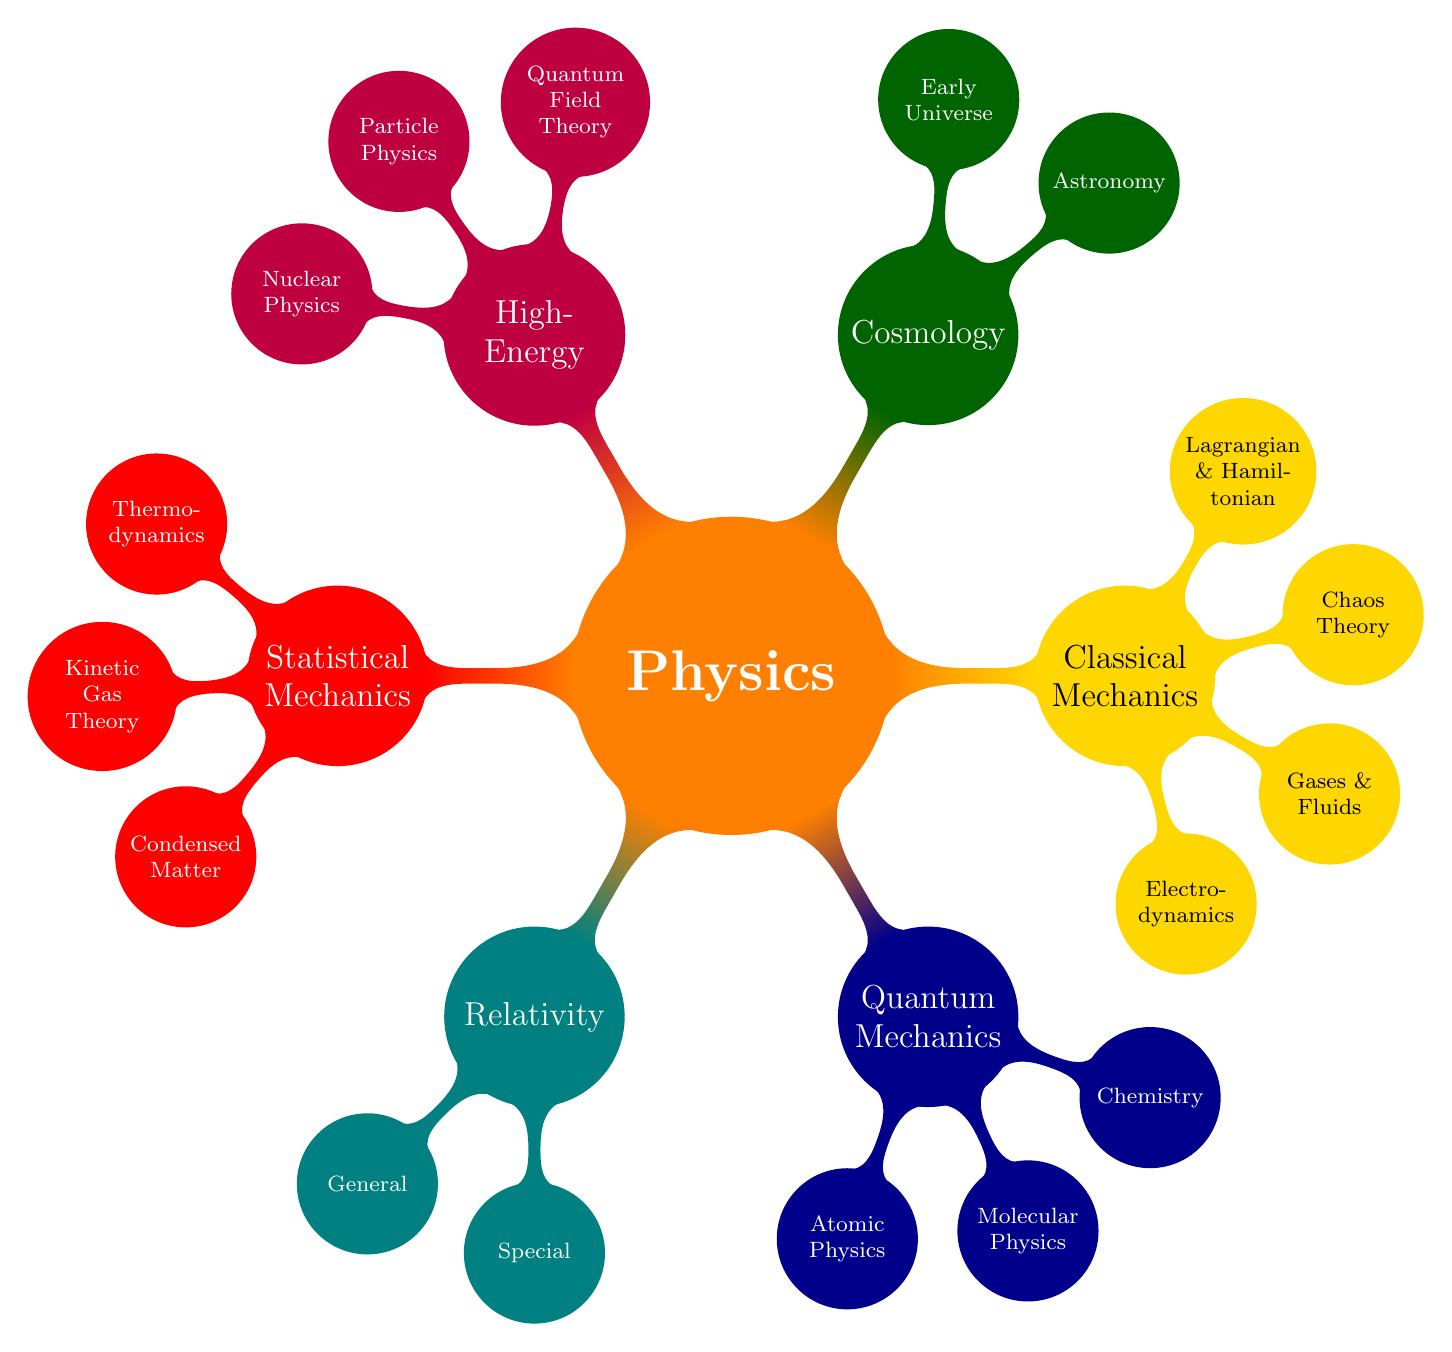
\begin{tikzpicture}[
    mindmap, every node/.style=concept, concept color=orange, text=white,
    level 1/.append style={level distance=5cm, sibling angle=60, font=\large},
    level 2/.append style={level distance=3cm, sibling angle=45}
  ]

  \node{\textbf{\huge{Physics}}} [clockwise from=0]
  child [concept color=Gold, text=black] {
      node {Classical\\Mechanics} [clockwise from=60]
      child { node {Lagrangian \& Hamiltonian}}
      child { node {Chaos Theory}}
      child { node {Gases \& Fluids}}
      child { node {Electro\-dynamics}}
    }
  child [concept color=DarkBlue] {
      node {Quantum Mechanics} [counterclockwise from=250]
      child { node {Atomic Physics}}
      child { node {Molecular Physics}}
      child { node {Chemistry}}
    }
  child [concept color=teal] {
      node {Relativity} [clockwise from=270]
      child { node {Special}}
      child { node {General}}
    }
  child [concept color=red] {
      node {Statistical Mechanics} [counterclockwise from=140]
      child { node {Thermo\-dynamics}}
      child { node {Kinetic Gas Theory}}
      child { node {Condensed Matter}}
    }
  child [concept color=purple] {
      node {High-Energy} [counterclockwise from=80]
      child { node {Quantum Field Theory}}
      child { node {Particle Physics}}
      child { node {Nuclear Physics}}
    }
  child [concept color=DarkGreen] {
      node {Cosmology} [counterclockwise from=40]
      child { node {Astronomy}}
      child { node {Early Universe}}
    };
\end{tikzpicture}
\end{document}
